% ЕМТ 2022, VII клас — точен LaTeX препис от официалните файлове в Klasirane.com.
% Условия: https://klasirane.com/api/competitions/EMT/All/2022/7%20%D0%BA%D0%BB/probs
% SHA-256 (условия): cc9e83580ad9288883d60dad93d3291643257333c8a8da54b2ec7685dc8bd979
% Решения: https://klasirane.com/api/competitions/EMT/All/2022/7%20%D0%BA%D0%BB/sol
% SHA-256 (решения): a6975d8682ae030399d72453a70faed25ce29dd10f8e5ea335feedfeed747f95
% Mathpix Snip (условия): d533155a-ac85-40e2-b63c-db27e5eead4a
% Mathpix Snip (решения): de04f4de-76b4-4338-85de-8b9d59227c63
% Точковите оценки, правописът, формулировките и видимите печатни особености са запазени от източника.
% Фигурите са неизменни изрези от официалния PDF с решенията, изобразени при 300 dpi.
% PDF граници в точки (x, y, ширина, височина):
% 7-2-lemma-figure.png — стр. 2: (336, 364.8, 187.2, 216)
% 7-2-parallel-figure.png — стр. 2: (336, 628.8, 168, 139.2)
% 7-2-part-a-figure.png — стр. 3: (352.8, 132, 168, 163.2)
% 7-3-knight-board.png — стр. 4: (192, 124.8, 196.8, 206.4)
% 7-3-numbered-grid.png — стр. 4: (235.2, 523.2, 124.8, 93.6)

Задача 7.1. Възрастта на Борис сега е два пъти по-голяма от възрастта на Асен, когато Борис беше на толкова години, на колкото е Асен в момента. Когато Асен стане на сегашната възраст на Борис, тогава сборът на годините им ще бъде 45. На колко години е Асен сега?

Решение. Нека сега Асен е на $x$ години, а Борис сега е на $y$ години. ($0<x<y$)

$$
\begin{array}{|l|l|l|l|}
\hline
\text{Възраст на} & \text{Преди} & \text{Сега} & \text{След} \\
\hline
\text{Асен} & x-(y-x) & x & y \\
\hline
\text{Борис} & x & y & y+y-x \\
\hline
\end{array}
$$

Имаме
$$
\begin{gathered}
2(x-(y-x))=y \Longleftrightarrow 2(x-y+x)=y \Longleftrightarrow 2(2x-y)=y \Longleftrightarrow 4x-2y=y \Longleftrightarrow 4x=3y, \\
y+y+y-x=45 \Longleftrightarrow 3y-x=45.
\end{gathered}
$$

От $3y-x=45$ и $4x=3y$ следва, че $4x-x=45$, $3x=45$ и $x=15$. Следователно $y=20$. Сега Асен е на 15 години.

Критерии за оценяване.

1 т. за въведени неизвестни букви и ($0<x<y$); 1 т. за изразяване възрастта на Асен и Борис чрез въведените букви: преди, сега и след; 2 т. за съставяне на равенствата $2\cdot[x-(y-x)]=y$ и $y+y+y-x=45$; 1 т. за намиране на $x$ и $y$; 1 т. за отговор.

Задача 7.2. Даден е изпъкнал четириъгълник $ABCD$.

а) Триъгълниците $ABC$, $ABD$ и $ACD$ са остроъгълни и лицето на четириъгълника $ABCD$ е равно на $324\ \mathrm{cm}^{2}$. Ако $M$, $N$, $P$, $Q$, $E$, $F$ са средите съответно на отсечките $AB$, $BC$, $CD$, $DA$, $AC$, $BD$, намерете
$$
S_{MFQE}+S_{FNCP}.
$$
(Четириъгълникът $MFQE$ е вдлъбнат, а $FNCP$ е изпъкнал.)

б) Правите $AB$ и $CD$ са успоредни и диагоналите $AC$ и $BD$ се пресичат в точка $O$. Докажете, че
$$
S_{ABCD}^{2}+2\cdot S_{BOC}^{2}=S_{AOB}^{2}+S_{COD}^{2}+4\cdot S_{ABCD}\cdot S_{AOD}.
$$

Решение. Ще докажем следните помощни твърдения.

1. Ако $ABC$ е произволен триъгълник и $M$ и $N$ са точки съответно върху страните $AB$ и $AC$, то
$$
\frac{S_{AMN}}{S_{ABC}}=\frac{AM}{AB}\cdot\frac{AN}{AC}.
$$

Доказателство. Разглеждаме $ABN$. Имаме
$$
\frac{S_{AMN}}{S_{ABN}}=\frac{2S_{AMN}}{2S_{ABN}}=\frac{AM\cdot NN_{1}}{AB\cdot NN_{1}}=\frac{AM}{AB}
$$
и
$$
\frac{S_{ABN}}{S_{ABC}}=\frac{2S_{ABN}}{2S_{ABC}}=\frac{AN\cdot BB_{1}}{AC\cdot BB_{1}}=\frac{AN}{AC}.
$$

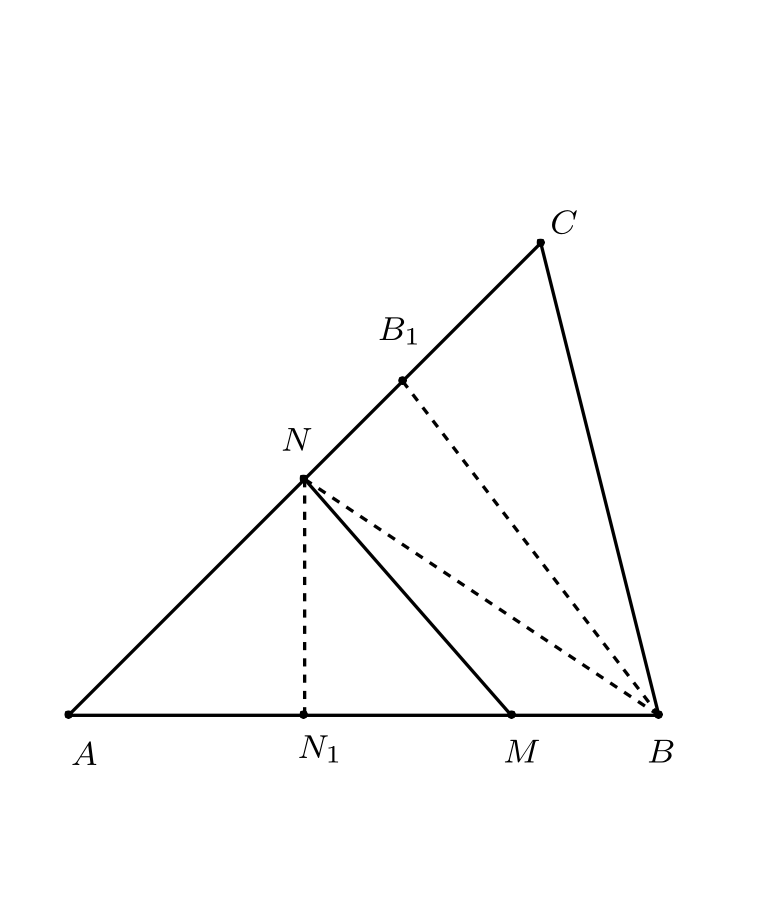
\includegraphics[max width=0.43\textwidth, alt={Триъгълник ABC с точки M и N и височини NN1 и BB1}, center]{assets/7-2-lemma-figure.png}

Следователно
$$
\frac{S_{AMN}}{S_{ABN}}\cdot\frac{S_{ABN}}{S_{ABC}}=\frac{AM}{AB}\cdot\frac{AN}{AC}\Longleftrightarrow\frac{S_{AMN}}{S_{ABC}}=\frac{AM}{AB}\cdot\frac{AN}{AC}.
$$

2. Ако правите $AB$ и $CD$ са успоредни, то $S_{ABC}=S_{ABD}$.

Доказателство. Тъй като $AB$ и $CD$ са успоредни, то $CC_{1}=DD_{1}$ и
$$
2S_{ABC}=AB\cdot CC_{1}=AB\cdot DD_{1}=2S_{ABD}.
$$

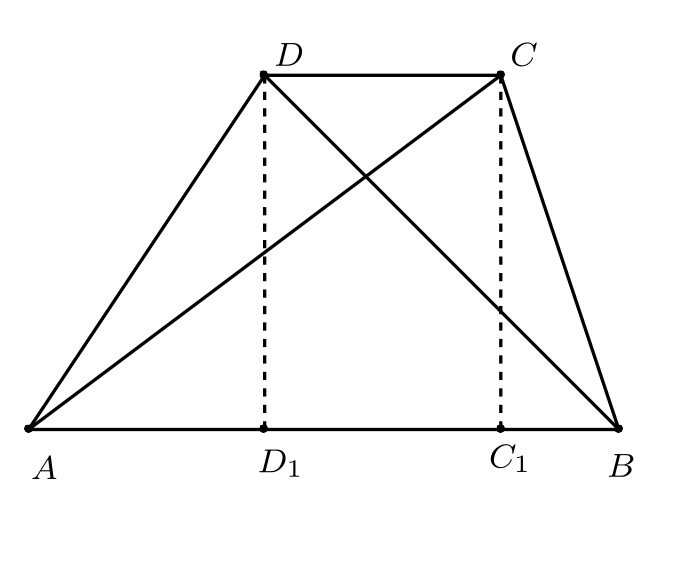
\includegraphics[max width=0.43\textwidth, alt={Трапец ABCD с диагонали и височини CC1 и DD1}, center]{assets/7-2-parallel-figure.png}

а) От условието, че триъгълниците $ABC$, $ABD$ и $ACD$ са остроъгълни следва, че четириъгълниците $AMEQ$, $BNFM$ и $DQFP$ нямат общи вътрешни точки. Следователно
$$
S_{MFQE}+S_{FNCP}+S_{AMEQ}+S_{BNFM}+S_{DQFP}=S_{ABCD}.
$$

Четириъгълниците $AMEQ$, $BNFM$ и $DQFP$ имат равни лица.
$$
S_{AMEQ}=S_{AME}+S_{AEQ}=\frac14S_{ABC}+\frac14S_{ACD}=\frac14S_{ABCD}.
$$

Аналогично се доказва, че $S_{BNFM}=\dfrac14S_{ABCD}$ и

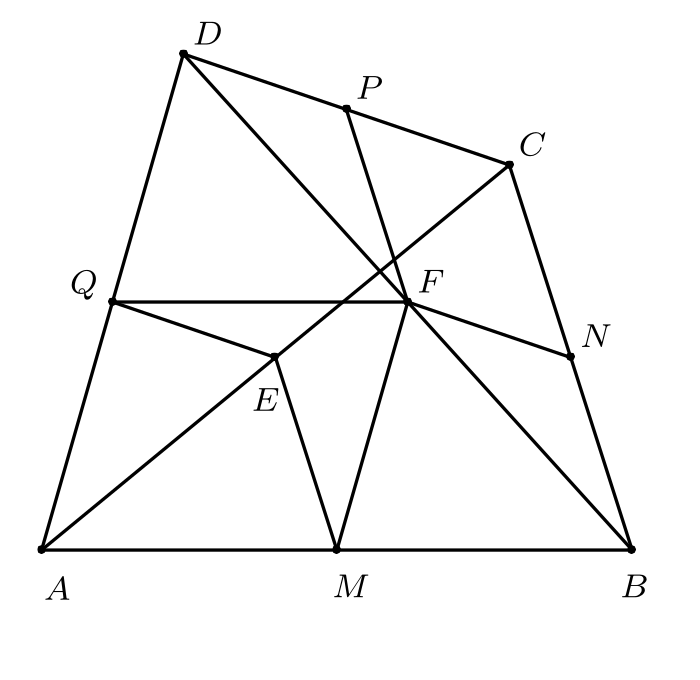
\includegraphics[max width=0.43\textwidth, alt={Четириъгълник ABCD със средите M N P Q E и F}, center]{assets/7-2-part-a-figure.png}

$S_{DQFP}=\dfrac14S_{ABCD}$. Следователно
$$
S_{MFQE}+S_{FNCP}=S_{ABCD}-\frac34S_{ABCD}=\frac14S_{ABCD}=81.
$$

б) Ще докажем, че $S_{AOB}\cdot S_{COD}=S_{BOC}\cdot S_{DOA}$.

Твърдението следва от
$$
\frac{S_{COD}}{S_{DOA}}=\frac{\frac12CO\cdot h_D}{\frac12AO\cdot h_D}=\frac{CO}{AO}=\frac{\frac12CO\cdot h_B}{\frac12AO\cdot h_B}=\frac{S_{BOC}}{S_{AOB}}.
$$

От $AB\parallel CD$ следва, че $S_{ABD}=S_{ABC}$, следователно $S_{ABO}+S_{AOD}=S_{ABO}+S_{BOC}$, т.е. $S_{AOD}=S_{BOC}$.

От $S_{ABCD}=S_{AOB}+S_{COD}+S_{BOC}+S_{AOD}=S_{AOB}+S_{COD}+2\cdot S_{BOC}$ следва, че
$$
S_{ABCD}^{2}+2\cdot S_{BOC}^{2}=\left(S_{AOB}+S_{COD}+2\cdot S_{BOC}\right)^{2}+2\cdot S_{BOC}^{2}=
$$
$$
\begin{gathered}
=S_{AOB}^{2}+S_{COB}^{2}+4\cdot S_{BOC}^{2}+2\cdot S_{AOB}\cdot S_{COD}+4\cdot S_{AOB}\cdot S_{BOC}+4\cdot S_{COD}\cdot S_{BOC}+2\cdot S_{BOC}^{2}= \\
=S_{AOB}^{2}+S_{COB}^{2}+4\cdot S_{BOC}^{2}+2\cdot S_{BOC}^{2}+4\cdot S_{AOB}\cdot S_{BOC}+4\cdot S_{COD}\cdot S_{BOC}+2\cdot S_{BOC}^{2}= \\
=S_{AOB}^{2}+S_{COB}^{2}+8\cdot S_{BOC}^{2}+4\cdot S_{AOB}\cdot S_{BOC}+4\cdot S_{COD}\cdot S_{BOC}= \\
=S_{AOB}^{2}+S_{COB}^{2}+4\left(2S_{BOC}^{2}+S_{AOB}\cdot S_{BOC}+S_{COD}\cdot S_{BOC}\right)= \\
=S_{AOB}^{2}+S_{COB}^{2}+4\left(2S_{BOC}+S_{AOB}+S_{COD}\right)\cdot S_{BOC}=S_{AOB}^{2}+S_{COB}^{2}+4S_{ABCD}\cdot S_{AOD}.
\end{gathered}
$$

Критерии за оценяване: а) 3 точки; б) 3 точки. (1 т. за $S_{AOB}\cdot S_{COD}=S_{BOC}\cdot S_{DOA}$ и $S_{AOD}=S_{BOC}$ и 2 т. за доказване на $S_{ABCD}^{2}+2\cdot S_{BOC}^{2}=S_{AOB}^{2}+S_{COD}^{2}+4\cdot S_{ABCD}\cdot S_{AOD}$.)

Задача 7.3. Най-много колко полета могат да се изберат върху шахматна дъска ($8\times8$) така, че от всяко избрано поле с един или два хода на коня да се стига до всяко от останалите избрани полета?

(За един ход конят се придвижва на две полета вертикално и след това едно хоризонтално, или на две полета хоризонтално и след това едно вертикално.)

Решение. Ако е поставен кон в поле D5, след 1-ви ход той може да бъде в полетата B4, B6, C3, C7, E3, E7, F4 и F6.

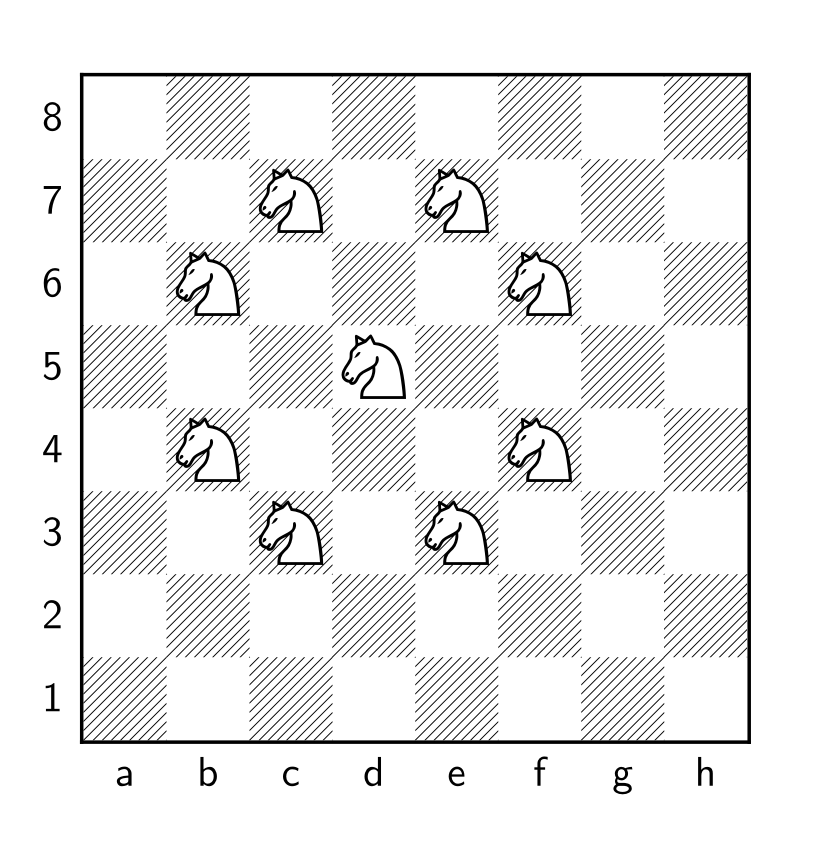
\includegraphics[max width=0.48\textwidth, alt={Шахматна дъска с кон в D5 и осемте полета на един ход от него}, center]{assets/7-3-knight-board.png}

Заедно с поле D5 имаме 9 полета. Тези 9 полета отговарят на условието, че между всеки две от тях може да се стигне с един или два хода на коня. Тези полета се намират в квадрат $5\times5$.

Да разгледаме най-лявото от отбелязаните полета $(X)$ и вертикалната ивица, която включва пет стълба, най-левият от които е този на $X$. Тази ивица съдържа всички отбелязани полета, тъй като не може да бъде напусната с два хода на коня, ако се тръгне от $X$. По същия начин, ако разгледаме най-горното от отбелязаните полета $(Y)$ и хоризонталната ивица, която включва пет реда, най-горният от които е редът на $Y$, тя съдържа всички отбелязани полета. Следователно всички отбелязани полета са в квадрата $5\times5$, който се получава при пресичането на двете ивици.

Ще покажем, че във всеки квадрат $5\times5$ не съществуват 10 полета, които отговарят на условието. Нека преномерираме полетата на квадрата с числата $1,2,3,\ldots,10$, както е показано на рисунката.

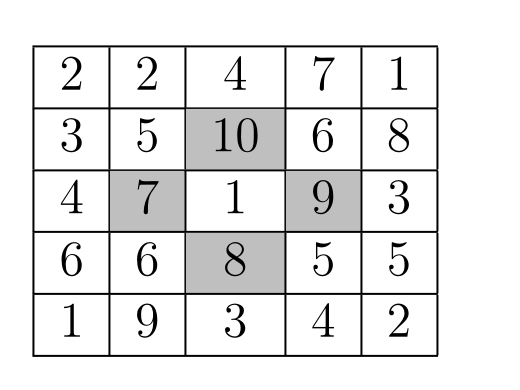
\includegraphics[max width=0.34\textwidth, alt={Номериран квадрат пет на пет с оцветени полета}, center]{assets/7-3-numbered-grid.png}

С числата от 1 до 6 са номерирани по 3 полета, с числата 7, 8 и 9 по 2 полета и с числото 10 едно поле. Забелязваме, че ако две полета са номерирани с едно и също число, то трябва да направим поне 3 хода с коня, за да отидем от едното поле в другото. Следователно при избор на 10 полета е необходимо те да са номерирани с различни числа. Полето с номер 10 ще е едно от избраните полета. Нека всяко от оцветените полета с номера 7, 8 и 9 е в избраните 10 полета. (Ако изберем вторите полета с номера 7, 8 и 9, разсъжденията са аналогични.) От останалите полета с номера от 1 до 6 се установява, че при всеки избор на едно от трите полета с един и същи номер, съществува поле от оцветените, до което се стига с три или повече хода на коня. Например ако от поле с номер 1 се стига с един ход до полета с номера 9 или 10, то от това поле до полетата с номера 7 или 8 се стига след 3 хода. Ако от поле с номер 1 се стига с един ход до полета с номера 7 или 8, то от това поле до полетата с номера 9 или 10 се стига след 3 хода. Аналогично с другите избори.

По този начин доказваме, че във всеки квадрат $5\times5$ от шахматната дъска не съществуват 10 полета, които да отговарят на условието. Следователно търсената най-голяма стойност е равна на 9.

Критерии за оценяване.

1 т. за посочване на 9 полета, които отговарят на условието; 1 т. за разглеждане на квадрат $5\times5$ с 9 полета, които отговарят на условието; 3 т. за преномериране полетата на квадрата $5\times5$; 2 т. за доказване, че не съществуват 10 полета.

Задача 7.4. а) Докажете, че ако $x$ и $y$ са естествени числа и стойността на израза
$$
M=\frac{x^{4}+y^{4}-x^{2}y^{2}}{(x+y)^{2}}
$$
е цяло число, то стойностите на изразите $\dfrac{xy}{x+y}$, $\dfrac{x^{2}}{x+y}$ и $\dfrac{y^{2}}{x+y}$ са естествени числа.

б) Намерете двойките естествени числа $(x;y)$, за които $x\leq y$, стойността на израза $\dfrac{xy}{x+y}$ е естествено число и $x+y\leq50$.

Решение. а) Преобразуваме числителя на $M$ по следния начин:
$$
x^{4}+y^{4}-x^{2}y^{2}=\left(x^{2}+y^{2}\right)^{2}-3x^{2}y^{2}=\left((x+y)^{2}-2xy\right)^{2}-3x^{2}y^{2}=(x+y)^{4}-4xy(x+y)^{2}+x^{2}y^{2}.
$$
Следователно $\left(\dfrac{xy}{x+y}\right)^{2}$ е естествено число и $\dfrac{xy}{x+y}$ също е естествено число. От равенството $xy=x(x+y)-x^{2}=y(x+y)-y^{2}$ получаваме, че $\dfrac{x^{2}}{x+y}$ и $\dfrac{y^{2}}{x+y}$ са естествени числа.

б) Нека $x=y$. Ако $\dfrac{xy}{x+y}$ е естествено число, то $\dfrac{xy}{x+y}=\dfrac{x^{2}}{2x}=\dfrac{x}{2}$, т.е. $x$ трябва да е четно число. Наистина, при $x=y=2t$, $t\in\mathbb{N}$ имаме $\dfrac{xy}{x+y}=\dfrac{4t^{2}}{4t}=t\in\mathbb{N}$.

Освен това, $2\leq x+y=4t\leq50$, т.е. $1\leq t\leq12$, което означава, че в този случай решенията са 12.

Нека $x+y$ дели $xy$, $x<y$ и НОД$(x;y)=d$. Следователно $x=dx_{1}$, $y=dy_{1}$, НОД$(x_{1},y_{1})=1$ и $x_{1}<y_{1}$. От доказателството на а) следва, че
$$
x+y\mid x^{2}\Longleftrightarrow d(x_{1}+y_{1})\mid d^{2}x_{1}^{2}\Longleftrightarrow x_{1}+y_{1}\mid dx_{1}^{2}.
$$
Аналогично и $x_{1}+y_{1}\mid dy_{1}^{2}$. Ако $p$ е просто число, което дели $x_{1}+y_{1}$, но не дели $d$, то $p\mid x_{1}$ и следователно $p\mid y_{1}$, а това е невъзможно. Остава $p$ да е делител на $d$. Щом като всеки прост делител на $x_{1}+y_{1}$ е делител на $d$ ще считаме, че $d=(x_{1}+y_{1})m$, $m\in\mathbb{N}$. Наистина, тогава
$$
\frac{xy}{x+y}=\frac{dx_{1}y_{1}}{x_{1}+y_{1}}=mx_{1}y_{1}\in\mathbb{N}.
$$

Освен това, от $x+y=d(x_{1}+y_{1})=m(x_{1}+y_{1})^{2}\leq50$ следва, че $3\leq x_{1}+y_{1}\leq7$. Разглеждаме тези случаи поотделно.

$$
\begin{array}{|c|c|c|c|c|}
\hline
x_{1}+y_{1} & x_{1} & y_{1} & m & \text{Брой двойки }(x;y) \\
\hline
3 & 1 & 2 & 1,2,3,4,5 & 5 \\
\hline
4 & 1 & 3 & 1,2,3 & 3 \\
\hline
5 & 1 & 4 & 1,2 & 2 \\
\hline
5 & 2 & 3 & 1,2 & 2 \\
\hline
6 & 1 & 5 & 1 & 1 \\
\hline
7 & 1 & 6 & 1 & 1 \\
\hline
7 & 2 & 5 & 1 & 1 \\
\hline
7 & 3 & 4 & 1 & 1 \\
\hline
\end{array}
$$

В този случай получаваме общо 16 двойки.

Окончателно, отговорът е $12+16=28$ двойки.

(Двойките с различни $x$ и $y$ са: $(3,6)$, $(4,12)$, $(6,12)$, $(5,20)$, $(6,30)$, $(7,42)$, $(8,24)$, $(9,18)$, $(10,15)$, $(10,40)$, $(12,24)$, $(12,36)$, $(14,35)$, $(15,30)$, $(20,30)$, $(21,28)$.)

Критерии за оценяване. а) 3 т. б) 4 т.
